% !TeX root = ../گزارش.tex
% !TeX encoding = UTF-8

% تجزیه وتحلیل، مروری برکارهای انجام شده، روش پیاده سازی |تحلیل و طراحی نرم افزار


\addcontentsline{toc}{section}{مقدمه}
\section*{مقدمه}
در این فصل به دیاگرام‌ها و سناریوهای نرم‌افزار پرداخته شده است.
\begin{figure}[H]
	\centering
	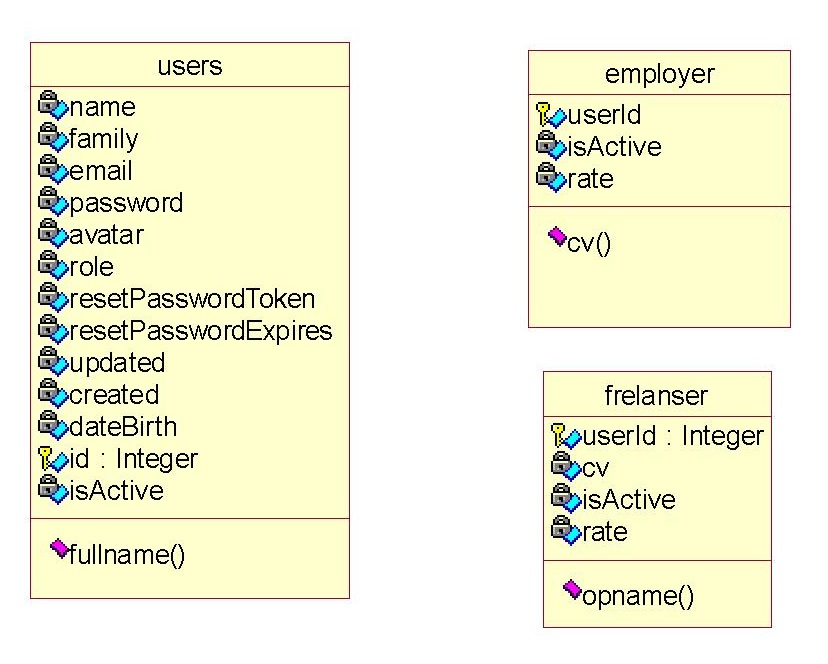
\includegraphics[width=0.7\textwidth]{Diagram/1.UseCase/کلی.jpg}
	\caption{دیاگرام UC ساختار کلی}
	\label{fig:uc:ساختار-کلی}
\end{figure}

\section{‌ثبت نام}

\textbf{مورد استفاده:}
ثبت‌نام
\\
\textbf{شرح مختصر :UC}
این قسمت مهمان در سایت ثبت‌نام می‌کند.
\\
\textbf{پيش شرط:}
 دانشجو باشد.
\\
\textbf{سناريو اصلی:}
\begin{enumerate}
\item
شروع
\item
مهمان دکمه ثبت‌نام را انتخاب می‌کند و سیستم فرم ثبت‌نام را به مهمان نمایش می‌دهد.
\item
مهمان فرم را تکمیل می‌کند و با دکمه ارسال، فرم تکمیل شده را به سیستم ارسال می‌کند.
\item
سیستم فرم ثبت‌نام را بررسی می‌کند و اطلاعات فرم را در بانک اطلاعات ثبت می‌کند.
\item
پایان
\end{enumerate}

\noindent
\textbf{پس شرط:}
ندارد.
\\
\textbf{سناريوهای فرعی:}
\\
\textbf{سناريو فرعی 1:}
خطا در اطلاعات وارد شده
\\
\textbf{شرح مختصر :UC}
این سناریو در مرحله ۴ سناریو اصلی در صورت خطا در اطلاعات وارد شده فرم ثبت‌نام اجرا می‌شود.
\begin{enumerate}
\item
شروع
\item
اطلاعات فرم بررسی می‌شود و خطاها مشخص می‌شوند.
\item
یک پیغام به مهمان نمایش داده می‌شود و درخواست اصلاح اطلاعات وارد شده را دارد.
\item
از مرحله 3 سناریو اصلی ادامه پیدا می‌کند.
\item
پایان
\end{enumerate}

\noindent
\textbf{سناريو فرعی 2:}
کاربر با موفقیت ایجاد شود.
\\
\textbf{شرح مختصر :UC}
این سناریو در مرحله ۴ سناریو اصلی در صورت موفقیت آمیز بودن ثبت‌نام اجرا می‌شود.
\begin{enumerate}
\item
شروع
\item
اطلاعات فرم بررسی می‌شود و یک پیغام به مهمان نمایش داده می‌شود که اطلاعات با موفقیت ثبت و کاربر ایجاد شده است.
\item
از مرحله 4 سناریو اصلی ادامه پیدا می‌کند.
\item
پایان
\end{enumerate}

\noindent
\textbf{سناريو فرعی 3:}
کاربر موجود باشد.
\\
\textbf{شرح مختصر :UC}
این سناریو در مرحله ۴ سناریو اصلی در صورت وجود کاربر در بانک اطلاعات اجرا می‌شود.
\begin{enumerate}
\item
شروع
\item
یک پیغام به مهمان نمایش داده می‌شود که اطلاعات کاربری از قبل وجود دارد و دکمه ورود به سایت نمایش داده می‌شود.
\item
پایان
\end{enumerate}

\noindent
\textbf{پس شرط:}
ندارد .


\begin{figure}[H]
	\centering
	\includegraphics[width=1\textwidth]{Diagram/2.Activity/ثبت‌نام.png}
	\caption{دیاگرام فعالیت ثبت‌نام}
	\label{fig:a:ثبت‌نام}
\end{figure}
\begin{figure}[H]
\centering
\includegraphics[width=1\textwidth]{Diagram/3.StateMachine/ثبت‌نام.png}
\caption{دیاگرام حالت ماشین ثبت‌نام}
\label{fig:sm:ثبت‌نام}
\end{figure}
\begin{figure}[H]
	\centering
	\includegraphics[width=1\textwidth]{Diagram/4.Collaboration/1.Sequence/ثبت‌نام.png}
	\caption{دیاگرام توالی ثبت‌نام}
	\label{fig:s:ثبت‌نام}
\end{figure}
\begin{figure}[H]
\centering
\includegraphics[width=1\textwidth]{Diagram/4.Collaboration/2.Communication/ثبت‌نام.png}
\caption{دیاگرام همکار ثبت‌نام}
\label{fig:c:ثبت‌نام}
\end{figure}


\section{ورود}
\documentclass[20pt,a5paper]{report}
\usepackage{graphicx,geometry}
\usepackage{multirow,hhline}
\usepackage[hidelinks]{hyperref}

\usepackage{xepersian}

\settextfont{Adobe Arabic}
\geometry{a5paper,top = 0.5cm, left = 1cm, right = 1cm, bottom = 0.5cm}


\begin{document}
\noindent \textbf{مورد استفاده:}
ورود
\\
\textbf{شرح مختصر :UC}
در این قسمت بازدیدکننده به سایت وارد میشود و به عنوان کاربر شناخنه میشود
\\
\textbf{پيش شرط:}
ثبت نام در سایت.
\\
\textbf{سناريو اصلی:}
\begin{enumerate}
\item 
شروع
\item 
بازدید کننده دکمه ورود را انتخاب میکند و سیستم فرم ورود را به بازدید کننده نمایش میدهد.
\item 
بازدید کننده فرم ورود را تکمیل میکند و با دکمه ارسال، فرم تکمیل شده را به سیستم ارسال میکند.
\item 
سیستم فرم ورود را بررسی میکند و اطلاعات را از بانک اطلاعات دریافت میکند .
\item 
کاربر در سایت شناسایی و وارد میشود٫
\item 
پایان
\end{enumerate}
\textbf{پس شرط:}
ندارد .
\\
\textbf{سناريوهای فرعی:}
\\ \\
\textbf{سناريو فرعی 1:}
خطا در اطلاعات فرم ورود
\\
\textbf{شرح مختصر :UC}
این سناریو در مرحله ۴ سناریو اصلی در صورت خطا در اطلاعات فرم ورود اجرا میشود.
\begin{enumerate}
\item 
شروع
\item 
اطلاعات فرم بررسی میشود و خطاها مشخص میشوند.
\item 
یک پیغام به بازدیدکننده نمایش داده میشود و درخواست اصلاح اطلاعات فرم را دارد.
\item 
از مرحله 3 سناریو اصلی ادامه پیدا میکند.
\item 
پایان
\end{enumerate}
\textbf{سناريو فرعی 2:}
کاربر با موفقیت وارد میشود.
\\
\textbf{شرح مختصر :UC}
این سناریو در مرحله ۴ سناریو اصلی در صورت موفقیت آمیز بودن ورود اجرا میشود.
\begin{enumerate}
\item 
شروع
\item 
اطلاعات فرم بررسی میشود و یک پیغام به کاربر نمایش داده میشود که ورود موفقیت آمیزی داشته.
\item 
از مرحله 5 سناریو اصلی ادامه پیدا میکند.
\item 
پایان
\end{enumerate}

\textbf{پس شرط:}
ندارد .


\centering
\vfill
\lr{\LaTeX}
\end{document}


\section{لیست پروژه‌ها}

\textbf{مورد استفاده:}
نمایش پروژه‌ها
\\
\textbf{شرح مختصر :UC}
نمایش پروژه‌های فعال در سایت.
\\
\textbf{پيش شرط:}
ندارد.
\\
\textbf{سناريو اصلی:}
\begin{enumerate}
\item
شروع
\item
مهمان دکمه پروژه‌ها را انتخاب می‌کند و سیستم کل پروژه‌ها را به مهمان نمایش می‌دهد.
\item
مهمان با انتخاب هر پروژه‌ به اطلاعات آن دسترسی پیدا می‌کند.
\item
پایان
\end{enumerate}

\noindent
\textbf{پس شرط:}
ندارد.
\\
\textbf{سناريوهای فرعی:}
\\
ندارد.
\\
\textbf{پس شرط:}
ندارد.


\begin{figure}[H]
	\centering
	\includegraphics[width=.7\textwidth]{Diagram/2.Activity/پروژه‌ها.png}
	\caption{دیاگرام فعالیت لیست پروژه‌ها}
	\label{fig:a:پروژه‌ها}
\end{figure}
\begin{figure}[H]
\centering
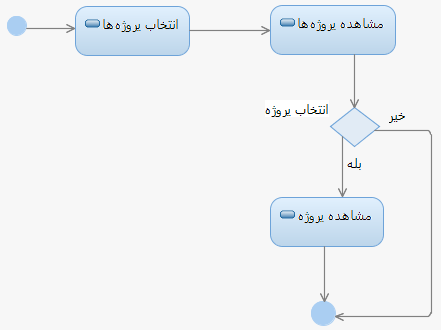
\includegraphics[width=.7\textwidth]{Diagram/3.StateMachine/پروژ‌ه‌ها.png}
\caption{دیاگرام حالت ماشین پروژه‌ها}
\label{fig:sm:پروژه‌ها}
\end{figure}
\begin{figure}[H]
	\centering
	\includegraphics[width=.5\textwidth]{Diagram/4.Collaboration/1.Sequence/پروژه‌ها.png}
	\caption{دیاگرام توالی پروژه‌ها}
	\label{fig:s:پروژه‌ها}
\end{figure}
\begin{figure}[H]
	\centering
	\includegraphics[width=.8\textwidth]{Diagram/4.Collaboration/2.Communication/پروژه‌ها.png}
	\caption{دیاگرام همکار پروژه‌ها}
	\label{fig:c:پروژه‌ها}
\end{figure}


\section{لیست فریلنسرها}

\textbf{مورد استفاده:}
نمایش فریلنسرها
\\
\textbf{شرح مختصر :UC}
نمایش فریلنسرهای فعال در سایت.
\\
\textbf{پيش شرط:}
ندارد.
\\
\textbf{سناريو اصلی:}
\begin{enumerate}
\item
شروع
\item
مهمان دکمه فریلنسرها را انتخاب می‌کند و سیستم فریلنسرها را به مهمان نمایش می‌دهد.
\item
مهمان با انتخاب هر فریلنسر به رزومه آن دسترسی پیدا می‌کند.
\item
پایان
\end{enumerate}

\noindent
\textbf{پس شرط:}
ندارد.
\\
\textbf{سناريوهای فرعی:}
\\
ندارد.
\\
\textbf{پس شرط:}
ندارد.


\begin{figure}[H]
	\centering
	\includegraphics[width=.7\textwidth]{Diagram/2.Activity/فریلنسرها.png}
	\caption{دیاگرام فعالیت فریلنسر‌ها}
	\label{fig:a:فریلنسر‌ها}
\end{figure}
\begin{figure}[H]
\centering
\includegraphics[width=.7\textwidth]{Diagram/3.StateMachine/فریلنسرها.png}
\caption{دیاگرام حالت ماشین فریلنسر‌ها}
\label{fig:sm:فریلنسر‌ها}
\end{figure}
\begin{figure}[H]
	\centering
	\includegraphics[width=.5\textwidth]{Diagram/4.Collaboration/1.Sequence/فریلنسرها.png}
	\caption{دیاگرام توالی فریلنسر‌ها}
	\label{fig:s:فریلنسر‌ها}
\end{figure}
\begin{figure}[H]
	\centering
	\includegraphics[width=.9\textwidth]{Diagram/4.Collaboration/2.Communication/فریلنسرها.png}
	\caption{دیاگرام همکار فریلنسر‌ها}
	\label{fig:c:فریلنسر‌ها}
\end{figure}



\section{داشبورد کاربر}
\textbf{مورد استفاده:}
داشبورد کاربر
\\
\textbf{شرح مختصر :UC}
در این قسمت دو داشبورد فریلنسر و کارفرما را در اختیار کاربر قرار می‌دهد.
\\
\textbf{پيش شرط:}
ورود به سایت.
\\
\textbf{سناريو اصلی:}
\begin{enumerate}
\item
شروع
\item
کاربر با انتخاب هر کدام از داشبوردها به عنوان کارفرما / فریلنسر به سیستم معرفی می‌شود.
\item
پایان
\end{enumerate}

\noindent
\textbf{پس شرط:}
ندارد .
\\
\textbf{سناريوهای فرعی:}
ندارد.
\\
\textbf{پس شرط:}
ندارد .


\begin{figure}[H]
	\centering
	\includegraphics[width=0.4\textwidth]{Diagram/1.UseCase/داشبورد-کاربر.png}
	\caption{دیاگرام UC داشبورد کاربر‌}
	\label{fig:uc:داشبورد-کاربر}
\end{figure}
\begin{figure}[H]
	\includegraphics[width=0.9\textwidth]{Diagram/2.Activity/داشبورد-کاربر.png}
	\centering
	\caption{دیاگرام فعالیت ‌داشبورد کاربر}
	\label{fig:a:داشبورد-کاربر}
\end{figure}
\begin{figure}[H]
\includegraphics[width=0.9\textwidth]{Diagram/3.StateMachine/داشبورد-کاربر.png}
\centering
\caption{دیاگرام حالت ماشین ‌داشبورد کاربر}
\label{fig:sm:داشبورد-کاربر}
\end{figure}
\begin{figure}[H]
	\includegraphics[width=1\textwidth]{Diagram/4.Collaboration/1.Sequence/داشبورد-کاربر.png}
	\caption{دیاگرام توالی ‌داشبورد کاربر}
	\centering
	\label{fig:s:داشبورد-کاربر}
\end{figure}
\begin{figure}[H]
\includegraphics[width=0.7\textwidth]{Diagram/4.Collaboration/2.Communication/داشبورد-کاربر.png}
\centering
\caption{دیاگرام همکار داشبورد کاربر}
\label{fig:c:داشبورد-کاربر}
\end{figure}


\section{داشبورد کارفرما}
\textbf{مورد استفاده:}
داشبورد کارفرما
\\
\textbf{شرح مختصر :UC}
در این قسمت داشبورد کارفرما را در اختیار کاربر قرار می‌دهد.
\\
\textbf{پيش شرط:}
ورود به داشبورد کارفرما.
\\
\textbf{سناريو اصلی:}
\begin{enumerate}
	\item
	شروع
	\item
	کارفرما به بخش‌های مختلف مانند ایجاد و اصلاح پروژه، انتخاب فریلنسر برای پروژه و .. دسترسی پیدا می‌کند.
	\item
	پایان
\end{enumerate}

\noindent
\textbf{پس شرط:}
ندارد.
\\
\textbf{سناريوهای فرعی:}
ندارد.
\\
\textbf{پس شرط:}
ندارد.


\begin{figure}[H]
	\centering
	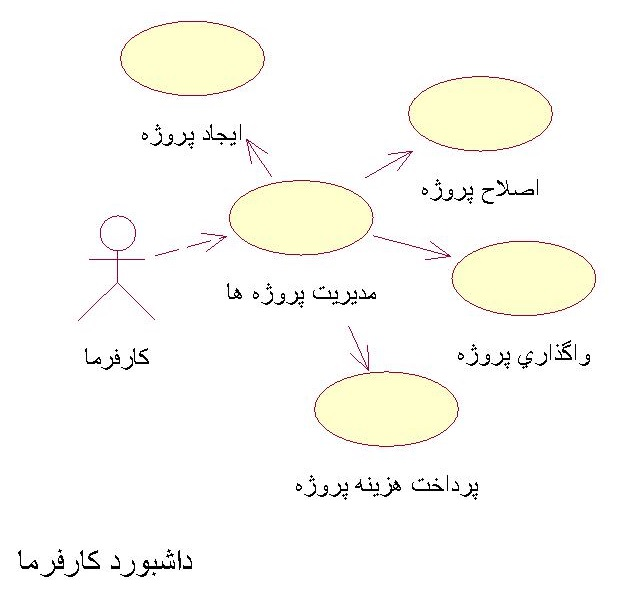
\includegraphics[width=.7\textwidth]{Diagram/1.UseCase/داشبورد-کارفرما.jpg}
	\caption{دیاگرام UC ‌داشبورد کارفرما}
	\label{fig:uc:داشبورد-کارفرما}
\end{figure}
\begin{figure}[H]
	\centering
	%\includegraphics[width=0.7\textwidth]{Diagram/4.Collaboration/-.jpg}
	\caption{دیاگرام همکار داشبورد کارفرما}
	\label{fig:c:داشبورد-کارفرما}
\end{figure}
\begin{figure}[H]
	\centering
	%\includegraphics[width=0.9\textwidth]{Diagram/2.Activity/-.jpg}
	\caption{دیاگرام فعالیت داشبورد کارفرما‌}
	\label{fig:a:داشبورد-کارفرما}
\end{figure}
\begin{figure}[H]
	\centering
	%\includegraphics[width=1\textwidth]{Diagram/3.Sequence/-.jpg}
	\caption{دیاگرام توالی ‌داشبورد کارفرما}
	\label{fig:s:داشبورد-کارفرما}
\end{figure}


\subsection{ایجاد پروژه}
\textbf{مورد استفاده:}
ایجاد پروژه
\\
\textbf{شرح مختصر :UC}
در این قسمت کارفرما پروژه خود را تعریف می‌کند.
\\
\textbf{پيش شرط:}
ورود به مدیریت پروژه در داشبورد کارفرما.
\\
\textbf{سناريو اصلی:}
\begin{enumerate}
\item
شروع
\item
کارفرما دکمه ایجاد پروژه را انتخاب می‌کند و سیستم فرم خام را به کارفرما نمایش می‌دهد.
\item
کارفرما فرم را تکمیل می‌کند و با دکمه ارسال، فرم تکمیل شده را به سیستم ارسال می‌کند.
\item
سیستم اطلاعات فرم را بررسی می‌کند و اطلاعات را در بانک اطلاعات ثبت می‌کند.
\item
پایان
\end{enumerate}

\noindent
\textbf{پس شرط:}
ندارد.
\\
\textbf{سناريوهای فرعی:}
\\
\textbf{سناريو فرعی 1:}
خطا در اطلاعات فرم ایجاد پروژه
\\
\textbf{شرح مختصر :UC}
این سناریو در مرحله ۴ سناریو اصلی در صورت خطا در اطلاعات فرم اجرا می‌شود.
\begin{enumerate}
\item
شروع
\item
اطلاعات فرم بررسی می‌شود و خطاها مشخص می‌شوند.
\item
یک پیغام به کارفرما نمایش داده می‌شود و درخواست اصلاح اطلاعات فرم را دارد.
\item
از مرحله 3 سناریو اصلی ادامه پیدا می‌کند.
\item
پایان
\end{enumerate}

\noindent
\textbf{سناريو فرعی 2:}
با موفقیت ثبت شود
\\
\textbf{شرح مختصر :UC}
این سناریو در مرحله ۴ سناریو اصلی در صورت موفقیت‌آمیز بودن ایجاد پروژه اجرا می‌شود.
\begin{enumerate}
\item
شروع
\item
اطلاعات فرم بررسی می‌شود و یک پیغام به کارفرما نمایش داده می‌شود که اطلاعات با موفقیت ثبت شده است.
\item
از مرحله 4 سناریو اصلی ادامه پیدا می‌کند.
\item
پایان
\end{enumerate}

\noindent
\textbf{پس شرط:}
ندارد.


\begin{figure}[H]
	\centering
	\includegraphics[width=.7\textwidth]{Diagram/2.Activity/کارفرما/مدیریت-پروژه-ایجاد.png}
	\caption{دیاگرام فعالیت ایجاد پروژه}
	\label{fig:a:ایجاد-پروژه}
\end{figure}
\begin{figure}[H]
\centering
\includegraphics[width=.7\textwidth]{Diagram/3.StateMachine/کارفرما/مدیریت-پروژه-ایجاد.png}
\caption{دیاگرام حالت ماشین ایجاد پروژه}
\label{fig:sm:ایجاد-پروژه}
\end{figure}
\begin{figure}[H]
	\centering
	\includegraphics[width=1\textwidth]{Diagram/4.Collaboration/1.Sequence/کارفرما/مدیریت-پروژه-ایجاد.png}
	\caption{دیاگرام توالی ایجاد پروژه}
	\label{fig:s:ایجاد-پروژه}
\end{figure}
\begin{figure}[H]
\centering
\includegraphics[width=.8\textwidth]{Diagram/4.Collaboration/2.Communication/کارفرما/مدیریت-پروژه-ایجاد.png}
\caption{دیاگرام همکار ایجاد پروژه}
\label{fig:c:ایجاد-پروژه}
\end{figure}


\subsection{ویرایش پروژه}
\textbf{مورد استفاده:}
ویرایش پروژه
\\
\textbf{شرح مختصر :UC}
در این قسمت کارفرما پروژه خود را اصلاح می‌کند.
\\
\textbf{پيش شرط:}
ورود به داشبورد کارفرما
\\
\textbf{سناريو اصلی:}
\begin{enumerate}
\item
شروع
\item
کارفرما دکمه ویرایش پروژه را انتخاب می‌کند و سیستم فرم اطلاعات پروژه را به کارفرما نمایش می‌دهد.
\item
کارفرما فرم را اصلاح می‌کند و با دکمه ارسال، فرم اصلاح شده را به سیستم ارسال می‌کند.
\item
سیستم اطلاعات فرم را بررسی می‌کند و اطلاعات را در بانک اطلاعات بروزرسانی می‌کند.
\item
پایان
\end{enumerate}

\noindent
\textbf{پس شرط:}
ندارد.
\\
\textbf{سناريوهای فرعی:}
\\
\textbf{سناريو فرعی 1:}
خطا در اطلاعات فرم ویرایش پروژه
\\
\textbf{شرح مختصر :UC}
این سناریو در مرحله ۴ سناریو اصلی در صورت خطا در اطلاعات فرم اجرا می‌شود.
\begin{enumerate}
\item
شروع
\item
اطلاعات فرم بررسی می‌شود و خطاها مشخص می‌شوند.
\item
یک پیغام به کارفرما نمایش داده می‌شود و درخواست اصلاح اطلاعات فرم را دارد.
\item
از مرحله 3 سناریو اصلی ادامه پیدا می‌کند.
\item
پایان
\end{enumerate}

\noindent
\textbf{سناريو فرعی 2:}
اطلاعات با موفقیت اصلاح شود
\\
\textbf{شرح مختصر :UC}
این سناریو در مرحله ۴ سناریو اصلی در صورت موفقیت آمیز بودن اصلاح اطلاعات پروژه اجرا می‌شود.
\begin{enumerate}
\item
شروع
\item
اطلاعات فرم بررسی می‌شود و یک پیغام به کارفرما نمایش داده می‌شود که اطلاعات با موفقیت ثبت شده است.
\item
از مرحله 4 سناریو اصلی ادامه پیدا می‌کند.
\item
پایان
\end{enumerate}

\noindent
\textbf{پس شرط:}
ندارد.



\begin{figure}[H]
	\centering
	\includegraphics[width=0.9\textwidth]{Diagram/2.Activity/داشبورد-کاربر/کارفرما/ویرایش-پروژه.jpg}
	\caption{دیاگرام فعالیت ویرایش پروژه}
	\label{fig:a:ویرایش-پروژه}
\end{figure}
\begin{figure}[H]
	\centering
	%\includegraphics[width=1\textwidth]{Diagram/3.Sequence/داشبورد-کاربر/کارفرما/ویرایش-پروژه.jpg}
	\caption{دیاگرام توالی ویرایش پروژه}
	\label{fig:s:ویرایش-پروژه}
\end{figure}
\begin{figure}[H]
\centering
%\includegraphics[width=0.7\textwidth]{Diagram/4.Collaboration/داشبورد-کاربر/کارفرما/ویرایش-پروژه.jpg}
\caption{دیاگرام همکار ویرایش پروژه}
\label{fig:c:ویرایش-پروژه}
\end{figure}


\subsection{پرداخت هزینه پروژه}
\textbf{مورد استفاده:}
پرداخت هزینه پروژه
\\
\textbf{شرح مختصر :UC}
در این قسمت کارفرما هزینه انجام پروژه توسط فریلنسر را پرداخت می‌کند.
\\
\textbf{پيش شرط:}
ورود به مدیریت مالی در داشبورد کارفرما.
\\
\textbf{سناريو اصلی:}
\begin{enumerate}
\item
شروع
\item
کارفرما بعد از انتخاب پروژه، دکمه پرداخت هزینه پروژه را انتخاب می‌کند و سیستم فرم پرداخت را به کارفرما نمایش می‌دهد.
\item
کارفرما فرم را تکمیل می‌کند و با دکمه ارسال، فرم تکمیل شده را به سیستم ارسال می‌کند.
\item
سیستم اطلاعات فرم را بررسی می‌کند و اطلاعات را به بانک عامل ارسال می‌کند.
\item
اطلاعات پرداخت دریافت می‌شود و در بانک اطلاعات ثبت می‌شود.
\item
پایان
\end{enumerate}

\noindent
\textbf{پس شرط:}
وجه بعد از انتخاب فریلنسر جهت ضمانت در سایت بلوکه می‌شود.
\\
\textbf{سناريوهای فرعی:}
\\
\textbf{سناريو فرعی 1:}
خطا در اطلاعات فرم پرداخت
\\
\textbf{شرح مختصر :UC}
این سناریو در مرحله 4 سناریو اصلی در صورت خطا در اطلاعات فرم اجرا می‌شود.
\begin{enumerate}
\item
شروع
\item
اطلاعات فرم بررسی می‌شود و خطاها مشخص می‌شوند.
\item
یک پیغام به کارفرما نمایش داده می‌شود و درخواست اصلاح اطلاعات فرم را دارد.
\item
از مرحله 3 سناریو اصلی ادامه پیدا می‌کند.
\item
پایان
\end{enumerate}

\noindent
\textbf{سناريو فرعی 2:}
خطا در پرداخت وجه
\\
\textbf{شرح مختصر :UC}
این سناریو در مرحله 5 سناریو اصلی در صورت خطا در پرداخت اجرا می‌شود.
\begin{enumerate}
\item
شروع
\item
اطلاعات خطا از طرف بانک عامل به سیستم ارسال می‌شود.
\item
یک پیغام به کارفرما نمایش داده می‌شود و ناموفق بودن پرداخت را اعلام می‌کند.
\item
از مرحله 2 سناریو اصلی ادامه پیدا می‌کند.
\item
پایان
\end{enumerate}

\noindent
\textbf{سناريو فرعی 3:}
با موفقیت پرداخت ‌شود
\\
\textbf{شرح مختصر :UC}
این سناریو در مرحله ۴ سناریو اصلی در صورت موفقیت آمیز بودن پرداخت اجرا می‌شود.
\begin{enumerate}
\item
شروع
\item
اطلاعات پرداخت از طرف بانک عامل به سیستم ارسال می‌شود.
\item
یک پیغام به کارفرما نمایش داده می‌شود که پرداخت با موفقیت انجام شده است.
\item
از مرحله 4 سناریو اصلی ادامه پیدا می‌کند.
\item
پایان
\end{enumerate}

\noindent
\textbf{پس شرط:}
ندارد.




\begin{figure}[H]
	\centering
	\includegraphics[width=.9\textwidth]{Diagram/2.Activity/کارفرما/مدیریت-مالی-پرداخت.png}
	\caption{دیاگرام فعالیت پرداخت هزینه}
	\label{fig:a:پرداخت-هزینه}
\end{figure}
\begin{figure}[H]
	\centering
	\includegraphics[width=.8\textwidth]{Diagram/3.StateMachine/کارفرما/مدیریت-مالی-پرداخت.png}
	\caption{دیاگرام حالت ماشین پرداخت هزینه}
	\label{fig:sm:پرداخت-هزینه}
\end{figure}
\begin{figure}[H]
	\centering
	\includegraphics[width=1\textwidth]{Diagram/4.Collaboration/1.Sequence/کارفرما/مدیریت-مالی-پرداخت.png}
	\caption{دیاگرام توالی پرداخت هزینه}
	\label{fig:s:پرداخت-هزینه}
\end{figure}
\begin{figure}[H]
	\centering
	\includegraphics[width=1\textwidth]{Diagram/4.Collaboration/2.Communication/کارفرما/مدیریت-مالی-پرداخت.png}
	\caption{دیاگرام همکار پرداخت هزینه}
	\label{fig:c:پرداخت-هزینه}
\end{figure}


\subsection{واگذاری پروژه}
\textbf{مورد استفاده:}
واگذاری پروژه
\\
\textbf{شرح مختصر :UC}
در این قسمت کارفرما پروژه را به یک فریلنسر واگذار می‌کند.
\\
\textbf{پيش شرط:}
ورود به مدیریت پروژه در داشبورد کارفرما.
\\
\textbf{سناريو اصلی:}
\begin{enumerate}
\item
شروع
\item
کارفرما دکمه قرارداد پروژه را انتخاب می‌کند و سیستم پیشنهادات فریلنسرها را به کارفرما نمایش می‌دهد.
\item
کارفرما بهترین پیشنهاد را انتخاب می‌کند و با دکمه تایید قرارداد را مشاهده کرده و وضعیت پیشنهاد را به سیستم ارسال می‌کند.
\item
سیستم به فریلنسر اطلاع داده و در بانک اطلاعات ثبت می‌کند.
\item
پایان
\end{enumerate}

\noindent
\textbf{پس شرط:}
فریلنسر باید برای ادامه قرارداد را تایید کند.
\\
\textbf{سناريوهای فرعی:}
ندارد.
\\
\textbf{پس شرط:}
ندارد.



\begin{figure}[H]
	\centering
	\includegraphics[width=.8\textwidth]{Diagram/2.Activity/کارفرما/مدیریت-پروژه-قرارداد-تایید.png}
	\caption{دیاگرام فعالیت واگذاری پروژه}
	\label{fig:a:واگذاری-پروژه}
\end{figure}
\begin{figure}[H]
\centering
\includegraphics[width=.8\textwidth]{Diagram/3.StateMachine/کارفرما/مدیریت-پروژه-قرارداد-تایید.png}
\caption{دیاگرام حالت ماشین واگذاری پروژه}
\label{fig:sm:واگذاری-پروژه}
\end{figure}
\begin{figure}[H]
	\centering
	\includegraphics[width=1\textwidth]{Diagram/4.Collaboration/1.Sequence/کارفرما/مدیریت-پروژه-قرارداد-تایید.png}
	\caption{دیاگرام توالی واگذاری پروژه}
	\label{fig:s:واگذاری-پروژه}
\end{figure}
\begin{figure}[H]
\centering
\includegraphics[width=0.7\textwidth]{Diagram/4.Collaboration/2.Communication/کارفرما/مدیریت-پروژه-قرارداد-تایید.png}
\caption{دیاگرام همکار واگذاری پروژه}
\label{fig:c:واگذاری-پروژه}
\end{figure}



\section{داشبورد فریلنسر}
\textbf{مورد استفاده:}
داشبورد فریلنسر
\\
\textbf{شرح مختصر :UC}
در این قسمت داشبورد فریلنسر را در اختیار کاربر قرار می‌دهد.
\\
\textbf{پيش شرط:}
ورود به داشبورد فریلنسر.
\\
\textbf{سناريو اصلی:}
\begin{enumerate}
	\item
	شروع
	\item
	فریلنسر به بخش‌های مختلف مانند ایجاد و اصلاح رزومه، پیشنهاد شرایط برای انجام پروژه کارفرما و .. دسترسی پیدا می‌کند.
	\item
	پایان
\end{enumerate}

\noindent
\textbf{پس شرط:}
ندارد.
\\
\textbf{سناريوهای فرعی:}
ندارد.
\\
\textbf{پس شرط:}
ندارد.


\begin{figure}[H]
	\centering
	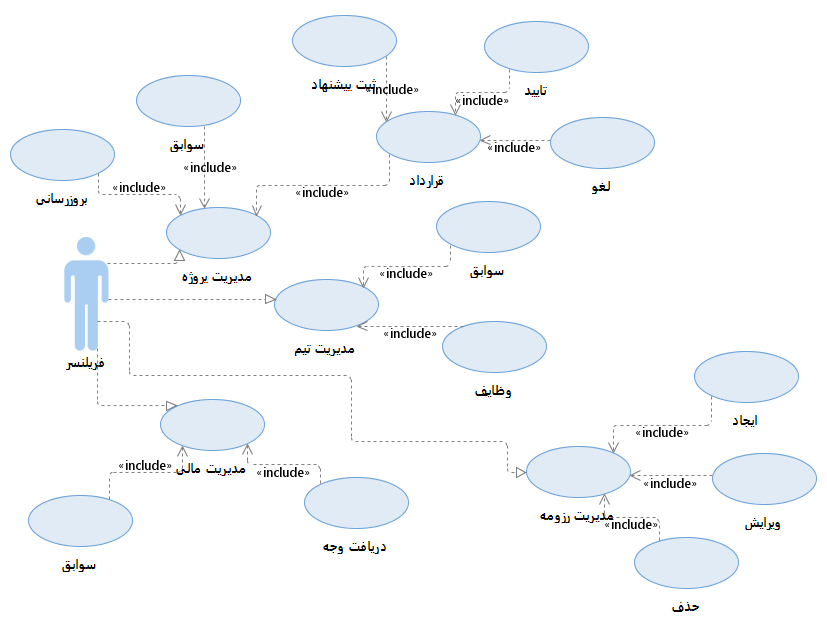
\includegraphics[width=0.7\textwidth]{Diagram/1.UseCase/داشبورد-فریلنسر.png}
	\caption{دیاگرام UC داشبورد فریلنسر}
	\label{fig:uc:داشبورد-فریلنسر}
\end{figure}

\subsection{ایجاد رزومه}
\textbf{مورد استفاده:}
ایجاد رزومه
\\
\textbf{شرح مختصر :UC}
در این قسمت فریلنسر رزومه خود را تعریف می‌کند.
\\
\textbf{پيش شرط:}
ورود به داشبورد فریلنسر.
\\
\textbf{سناريو اصلی:}
\begin{enumerate}
\item
شروع
\item
فریلنسر دکمه ایجاد رزومه را انتخاب می‌کند و سیستم فرم خام را به فریلنسر نمایش می‌دهد.
\item
فریلنسر فرم را تکمیل می‌کند و با دکمه ارسال، فرم تکمیل شده را به سیستم ارسال می‌کند.
\item
سیستم اطلاعات فرم را بررسی می‌کند و اطلاعات را در بانک اطلاعات ثبت می‌کند.
\item
پایان
\end{enumerate}

\noindent
\textbf{پس شرط:}
ندارد.
\\
\textbf{سناريوهای فرعی:}
\\
\textbf{سناريو فرعی 1:}
خطا در اطلاعات فرم ایجاد رزومه
\\
\textbf{شرح مختصر :UC}
این سناریو در مرحله ۴ سناریو اصلی در صورت خطا در اطلاعات فرم اجرا می‌شود.
\begin{enumerate}
\item
شروع
\item
اطلاعات فرم بررسی می‌شود و خطاها مشخص می‌شوند.
\item
یک پیغام به فریلنسر نمایش داده می‌شود و درخواست اصلاح اطلاعات فرم را دارد.
\item
از مرحله 3 سناریو اصلی ادامه پیدا می‌کند.
\item
پایان
\end{enumerate}

\noindent
\textbf{سناريو فرعی 2:}
رزومه با موفقیت ایجاد شود
\\
\textbf{شرح مختصر :UC}
این سناریو در مرحله ۴ سناریو اصلی در صورت موفقیت آمیز بودن ایجاد رزومه اجرا می‌شود.
\begin{enumerate}
\item
شروع
\item
اطلاعات فرم بررسی می‌شود و یک پیغام به فریلنسر نمایش داده می‌شود که اطلاعات با موفقیت ثبت شده است.
\item
از مرحله 4 سناریو اصلی ادامه پیدا می‌کند.
\item
پایان
\end{enumerate}

\noindent
\textbf{پس شرط:}
ندارد.



\begin{figure}[H]
	\centering
	\includegraphics[width=0.7\textwidth]{Diagram/2.Activity/داشبورد-کاربر/فریلنسر/ایجاد-رزومه.jpg}
	\caption{دیاگرام فعالیت ایجاد رزومه}
	\label{fig:a:ایجاد-رزومه}
\end{figure}
\begin{figure}[H]
	\centering
	\includegraphics[width=1\textwidth]{Diagram/3.Sequence/داشبورد-کاربر/فریلنسر/ایجاد-رزومه.jpg}
	\caption{دیاگرام توالی ایجاد رزومه}
	\label{fig:s:ایجاد-رزومه}
\end{figure}
\begin{figure}[H]
	\centering
	\includegraphics[width=0.7\textwidth]{Diagram/4.Collaboration/داشبورد-کاربر/فریلنسر/ایجاد-رزومه.jpg}
	\caption{دیاگرام همکار ایجاد رزومه}
	\label{fig:c:ایجاد-رزومه}
\end{figure}

\subsection{ویرایش رزومه}
\textbf{مورد استفاده:}
ویرایش رزومه
\\
\textbf{شرح مختصر :UC}
در این قسمت فریلنسر رزومه خود را ویرایش می‌کند.
\\
\textbf{پيش شرط:}
ورود به مدیریت رزومه در داشبورد فریلنسر.
\\
\textbf{سناريو اصلی:}
\begin{enumerate}
\item
شروع
\item
فریلنسر دکمه ویرایش رزومه را انتخاب می‌کند و سیستم فرم اطلاعات رزومه را به فریلنسر نمایش می‌دهد.
\item
فریلنسر فرم را اصلاح می‌کند و با دکمه ارسال، فرم اصلاح شده را به سیستم ارسال می‌کند.
\item
سیستم اطلاعات فرم را بررسی می‌کند و اطلاعات را در بانک اطلاعات بروزرسانی می‌کند.
\item
پایان
\end{enumerate}

\noindent
\textbf{پس شرط:}
ندارد.
\\
\textbf{سناريوهای فرعی:}
\\
\textbf{سناريو فرعی 1:}
خطا در اطلاعات فرم رزومه
\\
\textbf{شرح مختصر :UC}
این سناریو در مرحله ۴ سناریو اصلی در صورت خطا در اطلاعات فرم اجرا می‌شود.
\begin{enumerate}
\item
شروع
\item
اطلاعات فرم بررسی می‌شود و خطاها مشخص می‌شوند.
\item
یک پیغام به فریلنسر نمایش داده می‌شود و درخواست اصلاح اطلاعات فرم را دارد.
\item
از مرحله 3 سناریو اصلی ادامه پیدا می‌کند.
\item
پایان
\end{enumerate}

\noindent
\textbf{سناريو فرعی 2:}
رزومه با موفقیت ویرایش شود
\\
\textbf{شرح مختصر :UC}
این سناریو در مرحله ۴ سناریو اصلی در صورت موفقیت آمیز بودن ویرایش رزومه اجرا می‌شود.
\begin{enumerate}
\item
شروع
\item
اطلاعات فرم بررسی می‌شود و یک پیغام به فریلنسر نمایش داده می‌شود که اطلاعات با موفقیت ثبت شده است.
\item
از مرحله 4 سناریو اصلی ادامه پیدا می‌کند.
\item
پایان
\end{enumerate}

\noindent
\textbf{پس شرط:}
ندارد.



\begin{figure}[H]
	\includegraphics[width=0.7\textwidth]{Diagram/2.Activity/فریلنسر/مدیریت-رزومه-ویرایش.png}
	\centering
	\caption{دیاگرام فعالیت ویرایش رزومه}
	\label{fig:a:ویرایش-رزومه}
\end{figure}
\begin{figure}[H]
	\includegraphics[width=0.7\textwidth]{Diagram/3.StateMachine/فریلنسر/مدیریت-رزومه-ویرایش.png}
	\centering
	\caption{دیاگرام حالت ماشین ویرایش رزومه}
	\label{fig:sm:ویرایش-رزومه}
\end{figure}
\begin{figure}[H]
	\includegraphics[width=1\textwidth]{Diagram/4.Collaboration/1.Sequence/فریلنسر/مدیریت-رزومه-ویرایش.png}
	\caption{دیاگرام توالی ویرایش رزومه}
	\centering
	\label{fig:s:ویرایش-رزومه}
\end{figure}
\begin{figure}[H]
	\includegraphics[width=0.7\textwidth]{Diagram/4.Collaboration/2.Communication/فریلنسر/مدیریت-رزومه-ویرایش.png}
	\centering
	\caption{دیاگرام همکار ویرایش رزومه}
	\label{fig:c:ویرایش-رزومه}
\end{figure}


\subsection{درخواست پروژه}
\textbf{مورد استفاده:}
درخواست پروژه
\\
\textbf{شرح مختصر :UC}
در این قسمت فریلنسر پیشنهادات خود برای انجام پروژه را برای کارفرما ارسال می‌کند.
\\
\textbf{پيش شرط:}
ورود به مدیریت پروژه در داشبورد فریلنسر.
\\
\textbf{سناريو اصلی:}
\begin{enumerate}
\item
شروع
\item
فریلنسر دکمه درخواست پروژه را انتخاب می‌کند و سیستم فرم خام پیشنهاد به کارفرما را نمایش می‌دهد
\item
فریلنسر فرم را تکمیل می‌کند و با دکمه ارسال، اطلاعات را به سیستم ارسال می‌کند.
\item
سیستم اطلاعات را بررسی می‌کند و در بانک اطلاعات ثبت می‌کند.
\item
پایان
\end{enumerate}

\noindent
\textbf{پس شرط:}
کارفرما باید درخواست فریلنسر را تایید کند.
\\
\textbf{سناريوهای فرعی:}
\\
\textbf{سناريو فرعی 1:}
خطا در اطلاعات فرم درخواست پروژه
\\
\textbf{شرح مختصر :UC}
این سناریو در مرحله ۴ سناریو اصلی در صورت خطا در اطلاعات فرم اجرا می‌شود.
\begin{enumerate}
\item
شروع
\item
اطلاعات فرم بررسی می‌شود و خطاها مشخص می‌شوند.
\item
یک پیغام به فریلنسر نمایش داده می‌شود و درخواست اصلاح اطلاعات فرم را دارد.
\item
از مرحله 3 سناریو اصلی ادامه پیدا می‌کند.
\item
پایان
\end{enumerate}

\noindent
\textbf{سناريو فرعی 2:}
درخواست با موفقیت ثبت شود
\\
\textbf{شرح مختصر :UC}
این سناریو در مرحله ۴ سناریو اصلی در صورت موفقیت آمیز بودن ثبت درخواست پروژه اجرا می‌شود.
\begin{enumerate}
\item
شروع
\item
اطلاعات فرم بررسی می‌شود و یک پیغام به فریلنسر نمایش داده می‌شود که اطلاعات با موفقیت ثبت شده است.
\item
از مرحله 4 سناریو اصلی ادامه پیدا می‌کند.
\item
پایان
\end{enumerate}

\noindent
\textbf{پس شرط:}
ندارد.




\begin{figure}[H]
	\includegraphics[width=0.7\textwidth]{Diagram/2.Activity/فریلنسر/مدیریت-پروژه-قرارداد-ثبت-پیشنهاد.png}
	\centering
	\caption{دیاگرام فعالیت درخواست پروژه}
	\label{fig:a:درخواست-پروژه}
\end{figure}
\begin{figure}[H]
	\includegraphics[width=0.7\textwidth]{Diagram/3.StateMachine/فریلنسر/مدیریت-پروژه-قرارداد-ثبت-پیشنهاد.png}
	\centering
	\caption{دیاگرام حالت ماشین درخواست پروژه}
	\label{fig:sm:درخواست-پروژه}
\end{figure}
\begin{figure}[H]
	\includegraphics[width=1\textwidth]{Diagram/4.Collaboration/1.Sequence/فریلنسر/مدیریت-پروژه-قرارداد-ثبت-پیشنهاد.png}
	\caption{دیاگرام توالی درخواست پروژه}
	\centering
	\label{fig:s:درخواست-پروژه}
\end{figure}
\begin{figure}[H]
	\includegraphics[width=1\textwidth]{Diagram/4.Collaboration/2.Communication/فریلنسر/مدیریت-پروژه-قرارداد-ثبت-پیشنهاد.png}
	\centering
	\caption{دیاگرام همکار درخواست پروژه}
	\label{fig:c:درخواست-پروژه}
\end{figure}


\subsection{دریافت هزینه پروژه}
\textbf{مورد استفاده:}
دریافت هزینه انجام پروژه
\\
\textbf{شرح مختصر :UC}
در این قسمت فریلنسر هزینه پروژه را دریافت می‌کند.
\\
\textbf{پيش شرط:}
ورود به مدیریت مالی در داشبورد فریلنسر.
\\
\textbf{سناريو اصلی:}
\begin{enumerate}
\item
شروع
\item
فریلنسر دکمه دریافت هزینه پروژه را انتخاب می‌کند و پروژه  انجام شده را در سایت بارگذاری می‌کند.
\item
کارفرما پروژه را تست/رویت و نظر خود را با دکمه ثبت نظر ثبت می‌کند.
\item
پس از تایید/لغو طرفین، پول بلوکه شده آزاد و به حساب فریلنسر/کارفرما واریز می‌شود.
\item
پروژه خاتمه یافتنه و در بانک اطلاعات ثبت می‌شود.
\item
پایان
\end{enumerate}

\noindent
\textbf{پس شرط:}
ندارد.
\\
\textbf{سناريوهای فرعی:}
\\
\textbf{سناريو فرعی 1:}
اصلاحات پروژه
\\
\textbf{شرح مختصر :UC}
این سناریو در مرحله 3 سناریو اصلی کارفرما بخش‌های نیاز به اصلاح را به فریلنسر اعلام می‌کند.
\begin{enumerate}
\item
شروع
\item
اصلاحات مورد نظر کارفرما طبق جهارچوب و قوانین سایت به فریلنسر جهت اعمال اعلام می‌شود.
\item
از مرحله 3 سناریو اصلی ادامه پیدا می‌کند.
\item
پایان
\end{enumerate}

\noindent
\textbf{سناريو فرعی 2:}
شکایت
\\
\textbf{شرح مختصر :UC}
این سناریو در مرحله ۴ سناریو اصلی در صورت شکایت طرفین اجرا می‌شود.
\begin{enumerate}
\item
شروع
\item
یکی از طرفین دکمه ثبت شکایت را انتخاب می‌کند و توضیحات شکایت خود را ثبت می‌کند.
\item
کارشناسان سایت به پروژه ورود کرده و نظر خود را در رابطه با آن اعلام می‌کنند.
\item
پس از لغو/تایید پروژه، از مرحله ۴ سناریو اصلی ادامه پیدا می‌کند.
\item
پایان
\end{enumerate}

\noindent
\textbf{پس شرط:}
ندارد.



\begin{figure}[H]
	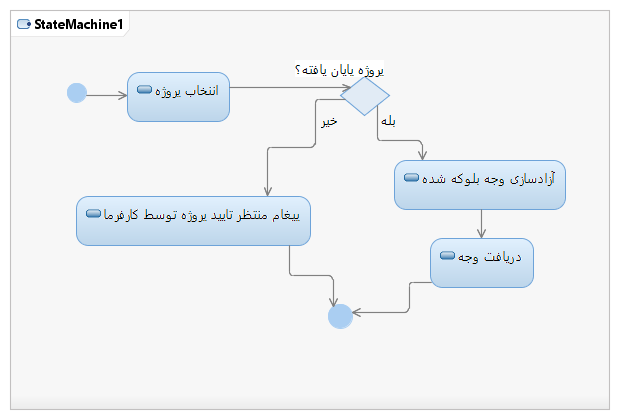
\includegraphics[width=1\textwidth]{Diagram/2.Activity/فریلنسر/مدیریت-مالی-دریافت-وجه.png}
	\centering
	\caption{دیاگرام فعالیت دریافت وجه}
	\label{fig:a:دریافت-وجه}
\end{figure}
\begin{figure}[H]
	\includegraphics[width=1\textwidth]{Diagram/3.StateMachine/فریلنسر/مدیریت-مالی-دریافت-وجه.png}
	\centering
	\caption{دیاگرام حالت ماشین دریافت وجه}
	\label{fig:sm:دریافت-وجه}
\end{figure}
\begin{figure}[H]
	\includegraphics[width=1\textwidth]{Diagram/4.Collaboration/1.Sequence/فریلنسر/مدیریت-مالی-دریافت-وجه.png}
	\caption{دیاگرام توالی دریافت وجه}
	\centering
	\label{fig:s:دریافت-وجه}
\end{figure}
\begin{figure}[H]
	\includegraphics[width=1\textwidth]{Diagram/4.Collaboration/2.Communication/فریلنسر/مدیریت-مالی-دریافت-وجه.png}
	\centering
	\caption{دیاگرام همکار دریافت وجه}
	\label{fig:c:دریافت-وجه}
\end{figure}



\section{داشبورد مدیریت}
\textbf{مورد استفاده:}
داشبورد مدیریت
\\
\textbf{شرح مختصر :UC}
در این قسمت داشبورد مدیریت را در اختیار مدیر قرار می‌دهد.
\\
\textbf{پيش شرط:}
ورود کاربر به سایت با سطح دسترسی مدیر.
\\
\textbf{سناريو اصلی:}
\begin{enumerate}
	\item
	شروع
	\item
	مدیر به بخش‌های مختلف مانند ایجاد و حذف کاربر، تعیین سطوح دسترسی کاربران و .. دسترسی پیدا می‌کند.
	\item
	پایان
\end{enumerate}

\noindent
\textbf{پس شرط:}
ندارد.
\\
\textbf{سناريوهای فرعی:}
ندارد.
\\
\textbf{پس شرط:}
ندارد.


\begin{figure}[H]
	\centering
	\includegraphics[width=0.7\textwidth]{Diagram/1.UseCase/داشبورد-مدیریت.jpg}
	\caption{دیاگرام UC داشبورد مدیریت}
	\label{fig:uc:داشبورد-مدیریت}
\end{figure}
\begin{figure}[H]
	%\includegraphics[width=0.1\textwidth]{Diagram/4.Collaboration/-.jpg}
	\centering
	\caption{دیاگرام همکار داشبورد مدیریت}
	\label{fig:c:داشبورد-مدیریت}
\end{figure}
\begin{figure}[H]
	%\includegraphics[width=0.7\textwidth]{Diagram/2.Activity/-.jpg}
	\centering
	\caption{دیاگرام فعالیت داشبورد مدیریت}
	\label{fig:a:داشبورد-مدیریت}
\end{figure}
\begin{figure}[H]
	%\includegraphics[width=0.7\textwidth]{Diagram/3.Sequence/-.jpg}
	\caption{دیاگرام توالی داشبورد مدیریت}
	\centering
	\label{fig:s:داشبورد-مدیریت}
\end{figure}


\subsection{مدیریت مالی}
\textbf{مورد استفاده:}
مدیریت مالی
\\
\textbf{شرح مختصر :UC}
در این قسمت مدیر می‌تواند تمام اطلاعات مالی را مشاهده ‌کند.
\\
\textbf{پيش شرط:}
ورود با کاربری مدیر
\\
\textbf{سناريو اصلی:}
\begin{enumerate}
	\item
	شروع
	\item
	مدیر دکمه مدیریت مالی را انتخاب می‌کند و گردش مالی، تاریخچه، ... را روئیت می‌کند.
	\item
	پایان
\end{enumerate}

\noindent
\textbf{پس شرط:}
ندارد.
\\
\textbf{سناريوهای فرعی:}
\\
ندارد



\subsection{شکایات/حل اختلاف}
\input{tex/Senario/مدیریت/شکایات}

\subsection{مدیریت کاربران}
\textbf{مورد استفاده:}
مدیریت  کاربران
\\
\textbf{شرح مختصر :UC}
در این قسمت مدیر می‌تواند تمام کاربران را مشاهده و بررسی ‌کند.
\\
\textbf{پيش شرط:}
ورود با کاربری مدیر
\\
\textbf{سناريو اصلی:}
\begin{enumerate}
	\item
	شروع
	\item
	مدیر دکمه مدیریت کاربران را انتخاب می‌کند و ایجاد، حذف، تعیین سطح دسترسی را روئیت می‌کند.
	\item
	پایان
\end{enumerate}

\noindent
\textbf{پس شرط:}
ندارد.
\\
\textbf{سناريوهای فرعی:}
\\
ندارد



\subsection{تنظیمات}
%در این پوشه تنظیمات نرم‌افزار قرار دارد. 

\begin{figure}[H]
	\includegraphics[width=.3\textwidth]{Folders-Files/config.png}
	\centering
	\caption{ساختار پوشه تنظیمات}
	\label{fig:folder-config}
\end{figure}

\paragraph{فایل expers}
در این فایل به تنظیمات فریم‌ورک اکسپرس که شامل ارتباط با پایگاه داده و فراخوانی فایل‌های .env و package پرداخته شده است. 

\paragraph{\rl{logInChecker}:}
اعتبارسنجی ورود کاربر به سایت.
\\
\textbf{توضیحات}
\hr
\begin{flushleft}
	\framebox[.9\textwidth][l]{
		\lr{
			\textcolor{type}{void}
			\textcolor{func}{logInChecker}
			\textcolor{symb}{(}
			\textcolor{type}{object}
			\textcolor{arg}{request}
			\textcolor{symb}{,}
			\textcolor{type}{object}
			\textcolor{arg}{response}
			\textcolor{symb}{,}
			\textcolor{type}{object}
			\textcolor{arg}{next}
			\textcolor{symb}{);}
		}
	}
\end{flushleft}
بررسی طلاعات کاربری و اعتبار زمانی.
\\
\textbf{پارامترها}
\hr \\[10pt]
\begin{tabular}{|m{4cm}|m{3cm}|m{10cm}|}
	\hline
	\multicolumn{1}{|c}{پارامتر}
	&
	\multicolumn{1}{|c}{نوع}
	&
	\multicolumn{1}{|c|}{توضیحات}
	\\
	\hline
	\multicolumn{1}{|c}{request}
	&
	\multicolumn{1}{|c|}{object}
	&
	نمایانگر درخواست HTTP و دارای خصوصیاتی برای درخواست رشته پرس‌و‌جو، پارامترها ، بدنه ، هدرهای HTTP و غیره است.
	در این اسناد و طبق قرارداد ، از این شی همیشه به عنوان req یاد می شود (و پاسخ HTTP res است).
	\\
	\hline
	\multicolumn{1}{|c}{response}
	&
	\multicolumn{1}{|c|}{object}
	&
	نمایانگر پاسخ HTTP که برنامه Express با دریافت درخواست HTTP ارسال می کند.
	در این اسناد و طبق قرارداد ، از شی همیشه به عنوان res یاد می شود (و درخواست HTTP req است).
	\\
	\hline
	\multicolumn{1}{|c}{next}
	&
	\multicolumn{1}{|c|}{object}
	&
	عملکرد میان‌افزار بعدی را نشان می دهد.
	\\
	\hline
\end{tabular}
\\[10pt]
\textbf{خروجی}
\hr \\
در صورتی که کاربر به سایت وارد شده باشد یا مهلت زمانی ورود کاربر به پایان نرسیده باشد برنامه ادامه می‌یابد، در غیر این صورت به صفحه ورود به سایت هدایت می‌شود.

